\documentclass[a4paper]{article}
\usepackage[T1]{fontenc}
\usepackage[utf8x]{inputenc}
\usepackage[italian]{babel}
\usepackage{graphicx}
\graphicspath{{figures/}} %Setting the graphicspath
\makeatletter
\providecommand*{\input@path}{}
\edef\input@path{{figures/}{}\input@path}% prepend
\makeatother
  \usepackage{multicol}
\usepackage{amsmath}
\numberwithin{equation}{section}% numera eq come #section.#formula
\usepackage{amsthm}
\usepackage{amssymb}
\usepackage{cancel}
\usepackage{subfigure}
\usepackage{mathtools}
\usepackage{esint}
\usepackage{float}
 \usepackage{import}
\usepackage{xcolor}
\usepackage{geometry}
\geometry{a4paper, top=2cm, bottom=2cm, left=2.5cm, right=2.5cm,  heightrounded, bindingoffset=5mm}
\setlength{\parindent}{0pt} %riduce l'indentazione dei paragrafi
% Quanto segue serve per inserire l'elenco di equazioni
\usepackage[subfigure]{tocloft}
 \newcommand{\listequationsname}{Elenco delle equazioni}
\newlistof{myequations}{equ}{\listequationsname}
\newcommand{\myequations}[1]{%
	\addcontentsline{equ}{myequations}{\protect\numberline{\theequation}#1}\par}
% aggiungere per ogni etichetta oltre \label anche \myequations{NOME}
\setlength{\cftmyequationsnumwidth}{2.3em}
\setlength{\cftmyequationsindent}{1.5em}


\usepackage{makeidx} %serve per fare l'indice analitico
% compilare il documento principale
% viene generato un file nome_file.idx
% aprire il file e andare su Strumenti -> Comandi -> \makeindex
% compilare nuovamente il documento iniziale
\makeindex
% aggiungere gli elementi con \index{NOME}
% \index{Voce ! Voce secondaria}

\renewcommand{\thesubsubsection}{}
%rimuove la numerazione dalle sotto-sotto sezione

\title{Formulario fisica tecnica}
\author{
	Mastrofini Alessandro\\
	\and
	Volpato Rebecca\\
}
\date{October 2021}

\begin{document}

\newpage
\maketitle
\newpage
\tableofcontents
\newpage	

\newpage 

Novità rispetto al programma:
\begin{itemize}
	\item Al posto degli esercizi sulla trasmissione del calore verranno raccontate alcune esperienze.
	\item 	\textbf{Orale}: tre domande di teoria (termodinamica, termofluidodinamica, termocinetica o trasporto di massa) 
	\item \textbf{Scritto}: due esercitazioni, una sulle miscele aria-vapore (studio del benessere ambientale, saper regolare ambienti in ambienti clinici), cicli frigoriferi, terza domanda semi teorica (raccontare una delle esercitazioni citate sopra). 
	\item Esercitazioni sulla criochirurgia, sulla termoregolazione del corpo umano, sul trasporto di massa in aorta aneurismatica, sul trasporto di massa nel circolo di Willis e sull’acustica ovvero rumore provocato dalle valvole stenotiche. 
	\item Non ci sono esercizi sulla trasmissione del calore e termofluidodinamica.
	\item Testo: Problematiche di fisica tecnica in ingegneria medica (9 capitoli, da Texmat). Risultati di lavori fatti da colleghi o in tesi di dottorato o nella tesi magistrale ecc.
	
\end{itemize}


\newpage 


\section{Termodinamica}
	 \index{Termodinamica}
\subsection{Introduzione}
	
parliamo delle termodinamica classica $\rightarrow$ Ottocentesca


La prima cosa che bisogna fare nella termodinamica classica è definire l’oggetto del nostro studio, cioè l’insieme dei corpi che vogliamo studiare e che chiameremo \textcolor{red}{sistema termodinamico} (insieme degli oggetti che vogliamo studiare), si decide quale sistema termodinamico si vuole studiare, ad esempio l’aria nella stanza.
Nel momento in cui decidiamo il sistema, decidiamo anche il contorno fisico del nostro sistema termodinamico S scelto arbitrariamente; quello che c’è all’interno del nostro sistema è l’oggetto del nostro studio, tutto il resto è l’esterno E, mentre S è all’interno del contorno fisico.
\textbf{Sistema termodinamico} : oggetto del nostro studio.
Vogliamo relazionare il sistema termodinamico, cioè quello che c’è all’interno, con l’esterno e in particolare ci interessa la relazione, ovvero le interazioni tra l’interno e l’esterno, cioè ci interessa quello che succede NEL sistema.

Consideriamo tre tipologie di scambi:
\begin{itemize}
	\item Scambi di massa (sistemi aperti)
	\item Scambi di lavoro (attraverso il contorno)
	\item Scambi di calore (attraverso il contorno)
\end{itemize}

Individuiamo quindi lo stato termodinamico del sistema univocamente con:
\begin{itemize}
	\item $M$, composizione chimica
	\item $p,v,T$ , variabili interne 
	\item $w,z$, variabili esterne (velocità e quota)
\end{itemize}

Sono ipotesi lontane dalla realtà poiché la termodinamica classica studia \underline{solo stati di equilibrio}. 


 
 \index{Lavoro}
Definizione fisica del \textbf{lavoro}: si parte dal sistema cilindro-pistone \begin{equation}
	l_i=\int_1^2 p_idv
\end{equation}
\label{lavoro}
\myequations{Lavoro}  

Lo so definisce a partire dal sistema cilindro-pistone al quale applichiamo una forza $F$. 

\textbf{Convenzione termodinamica}: lavoro positivo se fatto dal sistema verso l'esterno.

\textbf{Convenzione termodinamica}: calore positivo se assorbito dal sistema (convezione opposta al lavoro).

Ricordiamo che siamo in uno stato di equilibrio, ovvero il caso limite. 

Nell'esempio del palloncino affinché possa aumentare il volume dovremo essere nelle condizioni in cui il lavoro di dilatazione è trascurabile, $l_i=l_e+\cancel{l_d}$. Questo è possibile quando:
\begin{itemize}
	\item c'è equilibrio termodinamico interno
	\item $p_i=p_e$, altrimenti la differenza di pressione dilata il materiale
	\item Assenza di attriti
	\item $T_i=T_e$
\end{itemize}

Queste condizioni non sono mai realizzabili, l’importanza della termodinamica però è che è una scienza che ragiona al limite; lo scopo dell’ingegneria è quello di dire vediamo di ridurre l’importanza di queste differenze di pressione tra interno ed esterno.
\\

\textbf{Temperatura}: a partire dal \textit{termoscopio}scegliamo una funzione che dipende da una delle variabili del sistema $\theta_A=f0(x)$ e nel sistema internazionale scegliamo una funzione lineare: $f'(x)=ax=T_A$. Quindi si dimostra che la \textbf{temperatura empirica} $\theta _A$ è uguale alla \textbf{temperatura termodinamica} $T_A$. Fissando il punto triplo dell'acqua $T_T=273.16 \text{K}$ eliminiamo la costante incognita  $rightarrow  T=273.16 {\over x_T}$. Usando il punti fisso del ghiaccio e il punto fisso del vapore $rightarrow T_{v}-T_{g}=a\left(x_{v}-x_{g}\right) \Rightarrow \frac{T}{T_{v}-T_{g}}=\frac{x}{x_{v}-x_{g}} $. Nel  S.I.$T\left({ }^{\circ} C\right)=T(K)-273,15$


\subsection{Misure}

Grande intensive --> minuscole
Grandezze intensive --> maiuscole

Misura della pressione 

Il barometro misura la pressione assoluta $p_A=\rho g h$

Manometro differenziale: dislivello => differenza di pressione. Bilancio delle forze : $ \rho S+\rho S\Delta z g=p_AS+\rho_m S\Delta z g$
 
Allora si ottiene che la pressione del fluido in esame rispetto la pressione atmosferica è $\rho -\rho_A=\rho_m \Delta zg$ 

\subsection{Frigoriferi ad effetto termoelettrico}


Permettono di misurare la temperatura. 

\textbf{Effetto Seebeck}.Presi due metalli saldati alle estremità. Mettendo le due saldature a T diverse misuriamo un forza elettromotrice $\Delta E=f\left(T_A-T_B\right)=\alpha_{A B}\left(T_{A}-\mathrm{T}_{B}\right) $ dove l coefficiente di Seebeck dipende dai materiali ed è definito come $\alpha_{A B}:=\lim _{\Delta T \rightarrow 0} \frac{\Delta E}{\Delta T}=\frac{d E}{d T}$. Usato nei dispositivi di misura: termocoppie. 


\textbf{Effetto Peltier}. Due metalli dove passa corrente. Alla giunzione si osserva una cassione di calore $\dot Q$ proporzionale alla corrente per il coefficiente di Peltier: $\dot Q=\pi _{AB}I$. Legato anche al  coefficiente di Seebeck: $\pi_{AB}=\alpha_{A B} T$.


\textbf{Effetto Thompson} 
Corrente in un conduttore metallico $\Longrightarrow$ differenza di temperatura. La quantità di calore che viene scambiata con l’esterno è in valore
assoluto proporzionale alla corrente, alla differenza di temperatura e ad un coefficiente che è chiamato coefficiente di Thomson.
$$\left|d \dot{Q}_{T}\right|=|\tau I d T|=\left|\tau I \frac{d T}{d x} d x\right|$$ 

\begin{figure}[H]
	\begin{center}
		\subfigure[Seebeck]{
			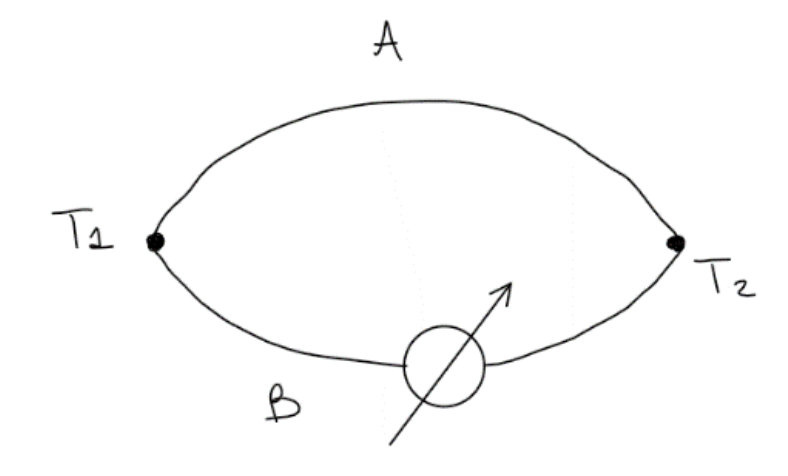
\includegraphics[height=0.15\columnwidth]{seebeck.png}}
		\subfigure[Peltier]{
			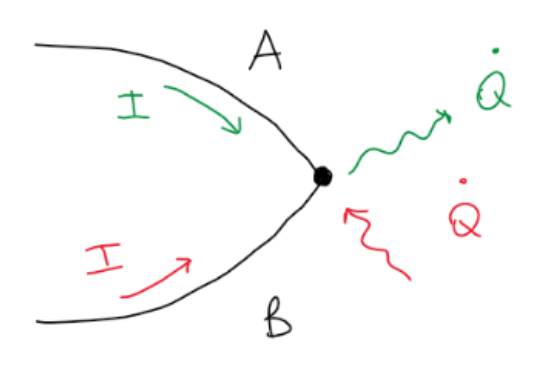
\includegraphics[height=0.15\columnwidth]{peltier.png}}
				\subfigure[Thompson]{
			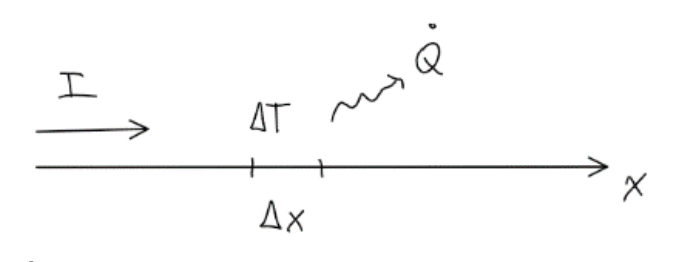
\includegraphics[height=0.15\columnwidth]{thompson.png}}
	\end{center}
				\caption{Frigoriferi a effetto termoelettrico}
\end{figure}


\subsection{Principio zero della termodinamica}

\textbf{Principio zero della termodinamica} o di Fowler. Presi due corpi A in equilibrio con C tramite una parete conduttrice. E il corpo B in equilibrio con lo stesso C. Allora, essendo entrambi in equilibrio con C, saranno A in equilibrio con B. $\Longrightarrow$ Possiamo usare C come termoscopio, per misurare se due corpi sono in equilibrio termico. 

\textbf{calore}
È l’interazione tra il sistema termodinamico e l’esterno, che avviene a causa di una differenza di temperatura, attraverso il contorno (tanto all’interno c’è equilibrio e non mi interessa). Questa definizione è generale, c'è anche quella operativa. 

\subsection{Primo principio della termodinamica}
 \index{Primo principio}
Il primo principio della termodinamica stabilisce che il lavoro scambiato in una trasformazione termodinamica {\color{red}{ciclica}} in un sistema {\color{red}{chiuso}} è uguale al calore totale scambiato: 
\begin{equation}
	L=Q
\end{equation}		
\label{primoprincipio}
\myequations{Primo principio della termodinamica}
Ricorda Esperienza di Joule e il fatto che lavoro e calore sono sono negativi (lavoro assorbito e calore ceduto) $-|L|=-|Q|$

Generalizzando vale l'uguaglianza integrale e quindi $dQ-dL=dE$ nota come \textbf{energia totale} e si tratta di una funzione di stato infatti $\oint dE=0$.

L'energia totale dipende da variabili interne e variabili esterne. $E=E_{interne}+E_{esterne}$
Tra le variabili esterne troviamo:
\begin{itemize}
	\item velocità del baricentro
	\item quota del baricentro
\end{itemize}
Allora $\Delta E_e=\Delta E_c+\Delta E_p$ (energia cinetica e potenziale).

Tra le variabili interne troviamo:
\begin{itemize}
	\item variabili termodinamiche (pressione, volume specifico, temperatura)
	\item componenti elettrochimiche (reazioni chimiche, fenomeni elettrici o termoelettrici)
\end{itemize}
Allora $\Delta E_i=\Delta u+\Delta u_x$ (energia interna termodinamica e energia interna di origine elettrochimica).

\textbf{Primo principio della termodinamica per un sistema chiuso che compie trasformazioni aperte}: 
 \index{Primo principio! trasf aperte in un sistema chiuso}
\begin{equation}
	Q-L=\Delta u+\Delta E_c +\Delta E_p 
\end{equation}
\label{1principio}
\myequations{Primo principio}

In termini differenziali:
\begin{equation}
	dq-dl=du+du_x+{dw^2\over 2}+g dz 
\end{equation}
\label{1principiodiff}
\myequations{Primo principio in termini differenziali}
 
\begin{figure}[h!]
	\begin{center}
		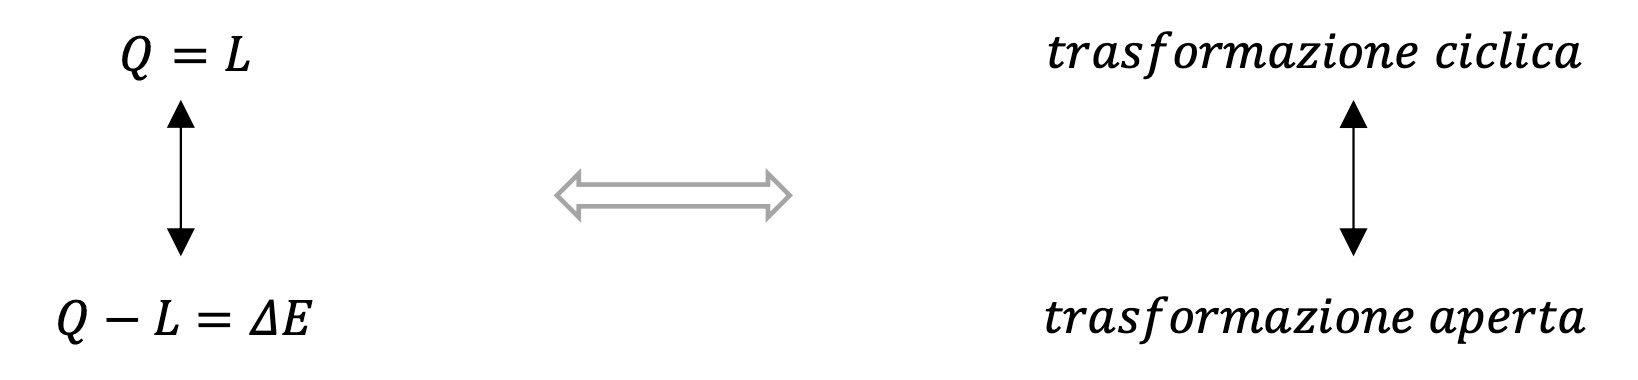
\includegraphics[width=0.6\columnwidth]{generalizprincipio.jpg}
	\end{center}
\end{figure}

\subsection{Sistemi aperti}
Lavoriamo in ipotesi di regime stazionario, in cui vale il bilancio di massa.
$M_t=M_{t+\Delta t}$
\begin{figure}[h!]
	\begin{center}
%		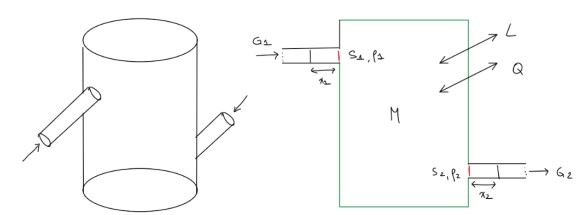
\includegraphics[width=0.6\columnwidth]{sistemaaperto.jpg}
		 \input{figures/sistemaperto.pdf_tex}
	\end{center}
\end{figure}


\textbf{bilancio di energia} $q-l_f-p_2v_2+p_1v_1=\Delta u + \frac{\Delta w^2}{2}+g\Delta z$

Dall'equazione del bilancio dell'energia entra in gioco una nuova grandezza funzione di stato: \textbf{Entalpia}: $h=u+pv$

\begin{equation}
	q-l_f=\Delta h +\Delta e_c + \Delta e_p
\end{equation}
\myequations{Primo principio per sistemi aperti}
Si definisce Entalpia come il calore scambiato in un sistema aperto dove non è presente lavoro e non ci sono variazioni di energia cinetica e di energia potenziale. $dq=dh$

\subsubsection{Espansore}
È un sistema aperto per produrre lavoro verso l'esterno. Il fluido si espando, diminuisce la pressione $\longrightarrow$ lavoro positivo (vedi \eqref{eq:lavorosistemiaperti}). 
\begin{figure}[H]
	\begin{center}
		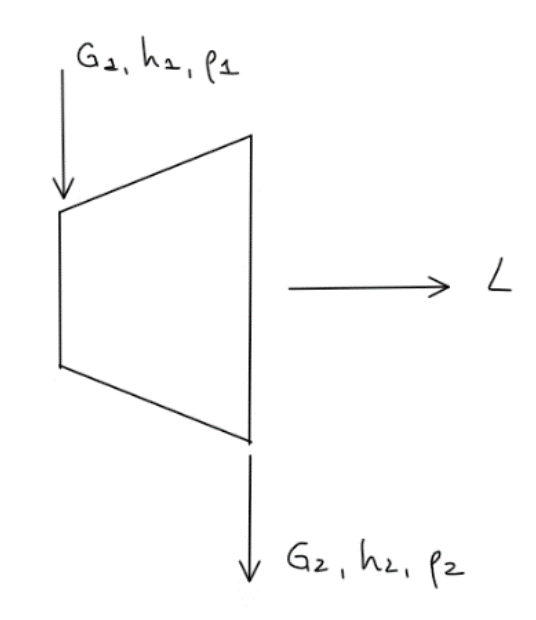
\includegraphics[width=0.2\columnwidth]{espansore.png}
	\end{center}
\end{figure}

Applichiamo il principio di conservazione della massa in regime stazionario e il principio di conservazione dell'energia (1° principio)  nel caso in cui $q=0$. Allora abbiamo \begin{equation}
	l_f=h_1-h_2>0
\end{equation}
\myequations{Lavoro dell'espansore}
Il fluido esce con un'entalpia minore. 

La potenza meccanica $P=l_f\cdot G_1=G\left(h_2-h_1\right)>0$

Il rendimento dell'espansore $\rho_{e}=\frac{l_{\text {reale }}}{l_{\text {ideale }}}=\frac{h_{1}-h_{2}}{\left(h_{1}-h_{2}\right)_{s}}$ , ha come limite superiore 1 (reversibilità). Nel caso ideale ($q=0$) consideriamo non ci siano cause di irreversibilità allora è una trasformazione adiabatica e reversibile $\Rightarrow$  isoentropica.

Quindi: $\rho_{e} \leq 1\begin{cases}
	=1 \text { per le trasformazioni reversibili } \\
	<1 \text { per le trasformazioni irreversibili reali }
\end{cases}$

\subsubsection{Compressore}

Con le stesse relazioni dell'espansore otteniamo un lavoro negativo (ceduto al sistema) 
\begin{equation}
	l_f=h_1-h_2<0
\end{equation}
\myequations{Lavoro del compressore}

\begin{figure}[H]
	\begin{center}
		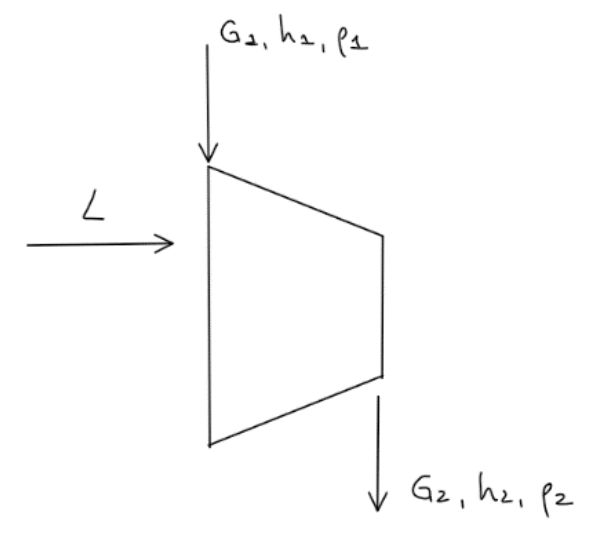
\includegraphics[width=0.2\columnwidth]{compressore.png}
	\end{center}
\end{figure}

C'è un aumento di entalpia dovuto al fatto che viene fornito lavoro al fluido $\Rightarrow$ aumento di pressione. $p_2>p_1$.

Analogamente per la potenza e il rendimento del compressore è il reciproco del rendimento dell'espansore. Il limite superiore è sempre 1 e valgono le stesse considerazioni dell'espansore. 

\subsubsection{Valvola di laminazione}

Non abbiamo scambi di calore ($q=0$) e $T_1=T_2$ e non c'è lavoro in quanto non c'è nessun organo meccanico che scambia lavoro. 

\begin{figure}[H]
	\begin{center}
				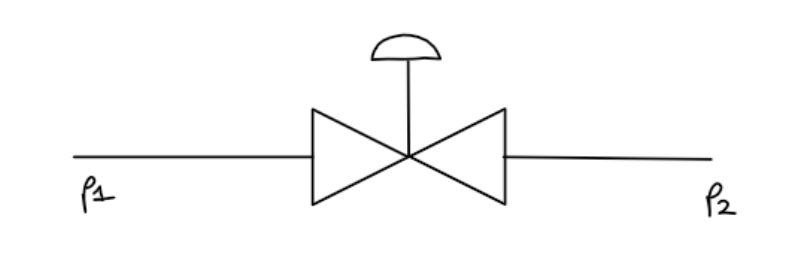
\includegraphics[width=0.3\columnwidth]{valvolalaminazione.png}
	\end{center}
\end{figure}

Allora dall'equazione del primo principio otteniamo
\begin{equation}
	\Delta h=0\Longrightarrow h_1=h_2
\end{equation}
\myequations{Valvola di laminazione}
È una tipica trasformazione \underline{irreversibile} poiché c'è un salto finito di pressione, cioè NON si parla di una trasformazione isoentalpica ma solo dell'uguglianza $h_1=h_2$. 

\subsubsection{Tubo di efflusso}

Riguarda la conversione dell'entalpia di un fluido in energia cinetica.

\begin{figure}[H]
	\begin{center}
		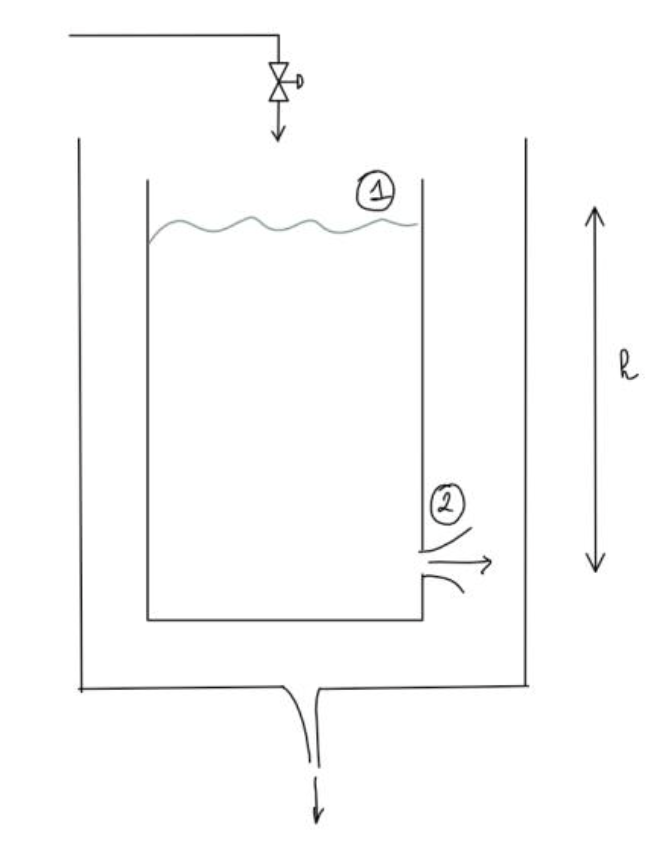
\includegraphics[width=0.3\columnwidth]{tuboefflusso.png}
	\end{center}
\end{figure}

Esperienza di Torricelli $\frac{w^{2}}{2 g}=h \rightarrow w=\sqrt{2 g h}$. 

Applicando il 1° principio (trascurando calore e lavoro) otteniamo $w_{2}^{2}=2 g\left(z_{1}-z_{2}\right)=2 g h$ da cui si torna al teorema di Torricelli.

\subsubsection{Generalizzazione dei sistemi aperti}

\begin{figure}[H]
	\begin{center}
		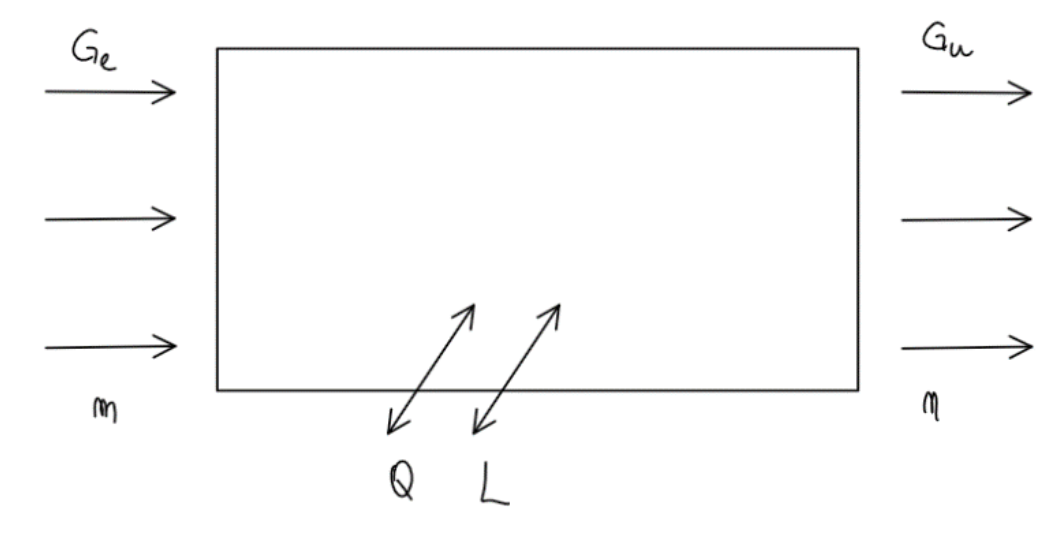
\includegraphics[width=0.5\columnwidth]{sistemiapertigen.png}
	\end{center}
\end{figure}

Siamo in regime stazionario. Vale il principio di conservazione della portata in massa $\sum_{e=1}^{m} G_{e}=\sum_{u=1}^{n} G_{u}$.

Vale il primo principio della termodinamica per i sistemi aperti e possiamo moltiplicarlo per le portate $G=G_1=G_2$.  Ovvero otteniamo:

\begin{equation}
	\dot{Q}-P_{f}=\sum_{u=1}^{n} G_{u}\left(h_{u}+e_{c u}+e_{p u}\right)-\sum_{e=1}^{m} G_{e}\left(h_{e}+e_{c e}+e_{p e}\right)
\end{equation}
\myequations{generalizzazione del 1° principio per i sistemi aperti}

Possiamo estenderla al regime \textcolor{red}{ non} stazionario:

  $\Longrightarrow$ la portata non si conserva: $\sum_{\rho} G_{e}-\sum_{u} G_{u}=\frac{d M}{d t}=\frac{M_{f}-M_{i}}{\Delta t}$
  
  Allora, applichiamo il primo principio della termodinamica considerando l'intervallo di tempo d'interesse ($\Delta t$), ovvero: 
  \begin{equation}
  	Q-L_{f}=\sum_{u} G_{u} \Delta t\left(h_{u}+e_{c u}+e_{p u}\right)-\sum_{e} G_{e} \Delta t\left(h_{e}+e_{c e}+e_{p e}\right)+M_{f} e_{t f}-M_{i} e_{t i}
  \end{equation}

Abbiamo aggiunto un termine che contiene l'energia totale (è variata sia l'energia potenziale che cinetica) e la quantità di massa che risulta variata. 



\subsection{Calore}
\index{Calore}
\textbf{Definizione operativa}: il calore si misura come il lavoro scambiato da un sistema in un'esperienza di Joule. Ovvero un sistema chiuso che compie una trasformazione ciclica. 

\subsection{Secondo principio della termodinamica}
 \index{Secondo principio}
\textbf{Formulazione di Plank}:
E' impossibile che l'unico risultato di una cessione di calore ad un sistema chiuso che compie trasformazioni cicliche sia la produzione di calore.

\textbf{Formulazione di Clausius}:
E' impossibile che per un sistema chiuso che compie trasformazioni cicliche l'unico risultato sia la sottrazione di calore da una sorgente inferiore e la cessione di calore ad una sorgente superiore senza alcun effetto compensatorio.

\begin{figure}[H]
	\begin{center}
		\caption{Macchina di Newcomen}
		%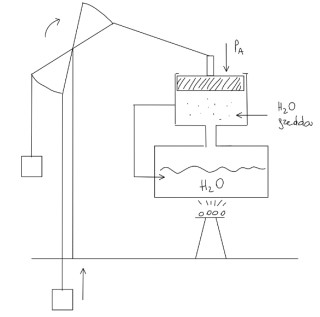
\includegraphics[width=0.4\columnwidth]{macchinaNewcomen.jpg}
				 \input{newcommen.pdf_tex}
	\end{center}
\end{figure}

Definiamo il rendimento come il rapporto tra ciò che si ottiene e ciò che si spende.
Questo meccanismo venne migliorato dalla macchina di Watt;

\begin{figure}[H]
	\begin{center}
		\caption{Macchina di Watt}
		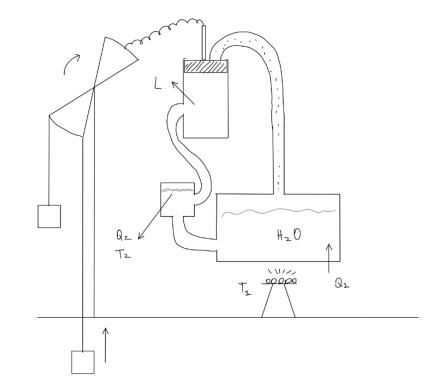
\includegraphics[width=0.6\columnwidth]{macchinadiWatt.jpg}
	\end{center}
\end{figure}

Distinguiamo il calore $Q_1$ che è il calore ceduto dal braciere al sistema termodinamico, il lavoro $L$ come il lavoro positivo esercitato dal sistema verso l'esterno e il calore $Q_2$ come il calore sottratto al sistema per ricondensare il vapore.

Per un sistema termodinamico chiuso che produce lavoro positivo grazie a scambi di calore il limite superiore del rendimento è il rendimento formulato da Carnot: $\eta_{max}=1-\frac{T_2}{T_1}$

\begin{figure}[H]
	\begin{center}
		\caption{Macchina motrice termica}
		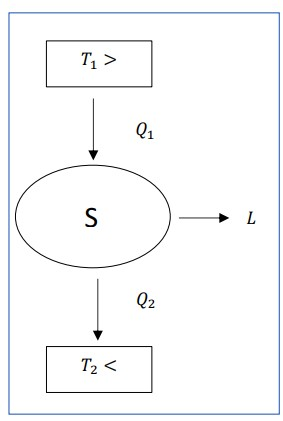
\includegraphics[width=0.2\columnwidth]{sistema.jpg}
	\end{center}
\end{figure}

Carnot fece una similitudine tra il mulino d'acqua e la macchina di Watt;
\begin{itemize}
	\item il lavoro L è lo stesso che produce in entrambi i casi una rotazione
	\item la quota coincide con la temperaturalatex d
	\item la portata coincide con il calore
\end{itemize}

il parallelismo errato era quello tra il calore e la portata perchè portava a scrivere $l=Q_1-Q_2=0$
Ma sappiamo che per produrre lavoro positivo la macchina di Watt deve avere $Q_1>Q_2$

Nei sistemi chiusi non si può invertire il segno del calore e del lavoro $\longrightarrow $ fenomeni sono \textbf{irreversibili}

\subsubsection{equivalenza dei principi}
 \index{Secondo principio! equivalenza}


\begin{figure}[H]
	\begin{center}
		\subfigure[Nego Plank]{
		\includegraphics[height=0.2\columnwidth]{Plank.jpg}}
		\subfigure[Nego Celsius]{
		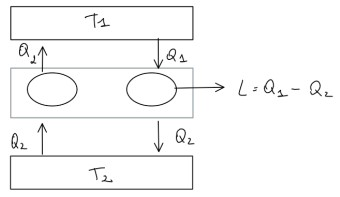
\includegraphics[height=0.2\columnwidth]{Clausius.jpg}}
				\caption{Uguaglianza delle formulazioni Planck, Clausius}
	\end{center}
\end{figure}

\subsection{Equazioni del secondo principio}
 \index{Secondo principio! equazioni}
\begin{equation}
	\oint \frac{dQ}{T} \le 0
\end{equation}
\myequations{Disuguaglianza di Clausius}
Questa viene chiamata \textbf{Disuguaglianza di Clausius}; dove T è la temperatura alla quale si scambia calore $dQ$. La disuguaglianza è:
\begin{itemize}
	\item $=0$ per trasformazioni reversibili
	\item $<$ per trasformazioni irreversibili
\end{itemize}

La disuguaglianza di Clausius cambiata di segno è la \textbf{Traccia termodinamica}

\textbf{ciclo diretto}
$\frac{Q_1}{T_1} - \frac{Q_2}{T_2} \le 0 \longrightarrow \frac{Q_{ass}}{T_{ass}} \le \frac{Q_{ced}}{T_[ced]}$

\textbf{ciclo inverso}
$-\frac{Q_1}{T_1} + \frac{Q_2}{T_2} \le 0 \longrightarrow \frac{Q_{ass}}{T_{ass}} \le \frac{Q_{ced}}{T_[ced]}$

Consideriamo la macchina negata della formulazione di Plank e verifichiamo che la disuguaglianza di Clausius sia negata; poichè il calore assorbito è positivo la disuguaglianza di Clausius risulta negata.

\subsection{Entropia}
\index{Entropia}
per una trasformazione reversibile $\oint \frac{dQ}{T}=0$
allora la grandezza $\frac{dQ}{T}=ds$: \textbf{Entropia}

se la trasformazione è irreversibile $\oint\frac{dQ}{T} \le 0$ e quindi possiamo scrivere:
$\frac{dQ}{T}=ds-ds_s$

\textbf{definizione operativa di entropia}
$\Delta s = s_2-s_1=\int_1^2\frac{dq}{T}$

Essendo una funzione di stato è uguale se calcolata lungo trasformazioni reversibili e irreversibili.

\subsubsection{Energia interna in funzione dell'entropia}
$dq-dl=du+de_c+de_p$
$du=dq-dl-de_c-de_p$  sappiamo che $dq=Tds$ e $dl=pdv$
\begin{equation}
	du=Tds-pdv
	\label{eq:energiainternaentropia}
\end{equation}
\myequations{Energia interna in funzione dell'entropia}

\subsubsection{Entalpia in funzione dell'entropia}
abbiamo definito $h=u+pv$, il differenziale è:
$dh=du+pdv+vdp$
dove $du=Tds-pdv$ quindi:

\begin{equation}
	dh=Tds+vdp
		\label{eq:entalpiaentropia}
\end{equation}
\myequations{Entalpia in funzione dell'entropia}

\subsubsection{Teorema dell'aumento di Entropia}\index{Entropia!teorema dell'aumento di entropia}
sistema termodinamico isolato con l'esterno, $dq=0$, allora $ds=ds_s$, quindi quando abbiamo trasformazioni irreversibili  il $ds_s$ va ad aumentare l'entropia. 
$ds_s \longrightarrow$ termine di produzione entropica

\subsubsection{Sorgenti di produzione entropica}\index{Entropia!sorgenti entropiche}
\begin{itemize}
	\item sorgenti entropiche di prima specie: cause di irreversibilità di prima specie quali differenza di pressione, di temperatura e attriti.
	\item sorgenti entropiche di seconda specie: irreversibilità di prima specie dovute a fenomeni elettrochimici
\end{itemize}

\begin{equation}
	ds_s=ds_{sI}(\Delta p, \Delta T, attriti)+ds_{sII}(x_i,l_{el})
\end{equation}
\label{sorgentientropiche}
\myequations{Sorgenti entropichei}

$dS=dQ\left(\frac{1}{T_2}-\frac{1}{T_1}\right)=dS_{sI}(\Delta T)>0$

$ds_{sI}=(\Delta p)=-\frac{vdp}{T}$

Per le cause di irreversibilità di seconda specie, consideriamo la variazione di energia interna elettrochimica $d u_{x}=\left(\frac{\partial e_{i}}{\partial x}\right) d x=X d x$ cioè  $d u_{x}=-d l_{e l}-T d s_{s I I}$. La $x$ rappresenta il grado di avanzamento della reazioni chimica e $dx$ la sua variazione.

Dissipata sotto forma di lavoro elettrico (il '-' per analogia con il 1° principio) o di irreversibilità ($Tds_{II}$ ), il '-' in analogia al calore, noto come calore dissipato non utilizzato a causa delle irreversibilità).

Quindi la sorgente entropica di seconda specie è: 
\begin{equation}
d s_{S I I}=\frac{1}{T}\left(-d u_{x}-d l_{e l}\right)=-\frac{d l_{e l}}{T}-\frac{X d x}{T}\text{ (sist. chiusi)}
\end{equation}
\label{sorgentientropiche2sistchiusi}
\myequations{Sorgenti entropiche di seconda specie per i sistemi chiusi}

Ragionando per i sist. aperti consideriamo la variazione di entalpia: $d h_{t}=d h+d h_{x}$ con un contributo termodinamico e uno della reazione elettrochimica. $\Longrightarrow$ $d h_{x}=\left(\frac{\partial h_{t}}{\partial x}\right) d xXx^{\prime} d x$. Quindi consideriamo che la variazione può dar luogo a lavoro elttrodico o sorgente entropica di seconda specie $d h_{x}=-d l_{e l}-T d s_{s I I}$.

In conclusione, la sorgente entropica di seconda specie: 
\begin{equation}
d s_{S I I}=-\frac{d l_{e l}}{T}-\frac{x^{\prime} d x}{T}\text{ (sist. aperti)}
\label{eq:sorgentientropiche2sistaperti}
\end{equation}
\myequations{Sorgenti entropiche di seconda specie per i sistemi aperti}

\subsubsection{Lavoro meccanico in presenza di sorgenti entropiche (trasformazioni irreversibili)}

 
\textbf{Sistemi chiusi}
Inseriamo le sorgenti entropiche nel 1° principio della termodinamica aggiungendo al lavoro il termine elettrico $dl_t=dl_m+dl_{ell}$ . Quindi dal 1° principio abbiamo che $du_t=dq-dl_t$ ma $du_t=du+du_x$ e per $dq=Tds-Td{s_s}$. Allora, sfruttando l'equazione  $d u_{x}=-d l_{e l}-T d s_{s I I}$  e \eqref{eq:energiainternaentropia}  otteniamo:

\begin{equation}
	dl_m=pdv-Tds_{sI}
	\label{eq:lavorosistemichiusi}
\end{equation}
\myequations{Lavoro per sistemi aperti}

Il lavoro meccanico è diminuito a causa delle irreversibilità di prima specie. 
\\

\textbf{Sistemi aperti}
Partendo dal primo principiamo consideriamo il lavoro con anche i fenomeni elettrici. Abbiamo $dh_t=dq-dl_t$ e $dh_t=dh+dh_x$ e che che $dq=Tds-Tds_s$. Sostituendo e ricordando che \eqref{eq:entalpiaentropia}  e che $d h_{x}=-d l_{e l}-T d s_{s I I}$ otteniamo:
\begin{equation}
	dl_m=-vdp-Tds_{sI}
	\label{eq:lavorosistemiaperti}
\end{equation}
\myequations{Lavoro per sistemi chiusi}

Il lavoro meccanico reale è diminuito a causa delle irreversibilità di prima specie. 

In caso di sistema aperto con trasformazione reversibile per ottenere lavoro positivo il fluido si deve espandere e quindi la pressione deve diminuire $dp>0$. 

\subsection{Ciclo motore o ciclo diretto}\index{Ciclo motore}

Si intende un ciclo che produce lavoro positivo verso l'esterno. La rappresentazione schematica è il ciclo di Watt. 

\begin{figure}[H]
	\begin{center}

		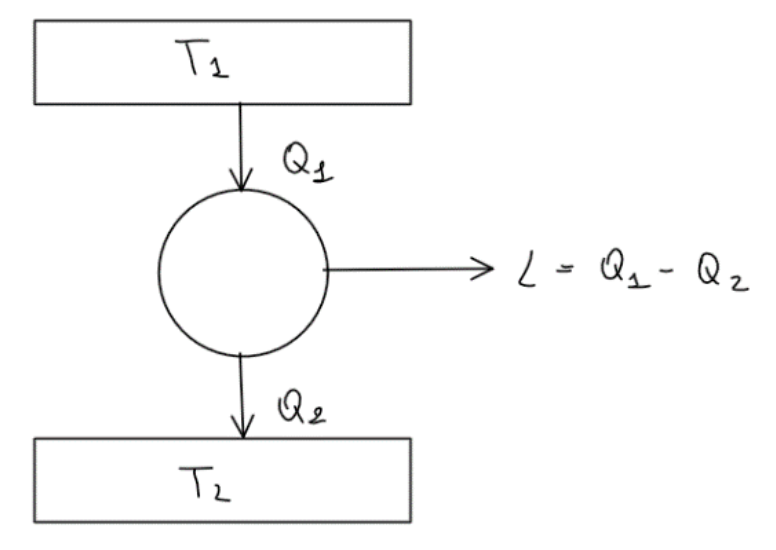
\includegraphics[width=0.3\columnwidth]{ciclomotore.png}
				\caption{Ciclo motore}
	\end{center}
\end{figure}

Otteniamo lavoro $L=Q_1-Q_2$.

Mettendo in relazione la traccia termodinamica (inverso della disugualianza di Clausius) ed il rendimento $\eta={L\over Q_1}={1-{Q_2\over Q_1}}$ otteniamo il rendimento del ciclo motore irreversibile 
\begin{equation}
	\eta=\left(1-{T_2\over T_1}\right)-\left. \tau T_2\over Q_1\right.
\end{equation}

Il primo termine corrisponde al rendimento massimo, ovvero quello di una macchina di Carnot (trasformazione reversibile, $\tau =0$).

\subsubsection{Macchina di Carnot}\index{Ciclo motore! macchina di Carnot}

È reversibile ($p_1=p_2,T_1=T_2,$ no attriti).

Isoterme tra 1-2 e 3-4 (calore è l'area sottesa).

\begin{figure}[H]
	\begin{center}
		
		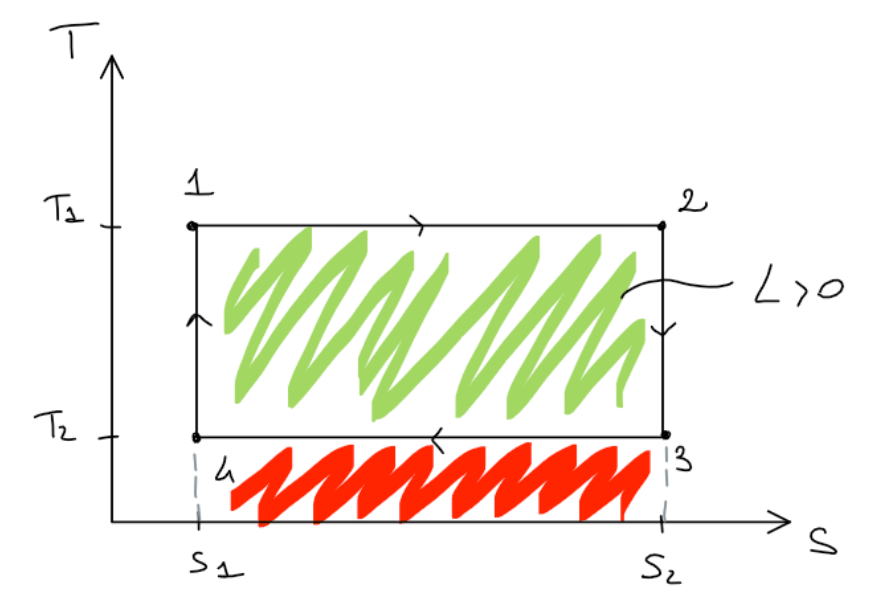
\includegraphics[width=0.4\columnwidth]{carnot.png}
		\caption{Ciclo motore}
	\end{center}
\end{figure}

Quindi abbiamo $d s=\frac{d q}{T}+d s_{S} \Rightarrow d s=0$ allora tra 2 -3 e 4-1 sono\textbf{ isoentropiche} (:=adiabatica reversibile).

È un ciclo motore particolare, infatti vale che il rendimento $\eta = \eta_c-f\left(\tau\right)$
N.B. Il rendimento di un ciclo termomeccanico massimo \textbf{non} è 1 ma $\eta_c =1-{T_2\over T_1}$

\subsection{Ciclo inverso}\index{Ciclo inverso}

\begin{itemize}
	\item ciclo frigorifero, se lo scopo è sottrarre $Q_2$ alla sorgente inferiore
	\item pompa di calore, se lo scopo è cedere $Q_1$ alla sorgente superiore
\end{itemize}


\begin{figure}[H]
	\begin{center}
		
		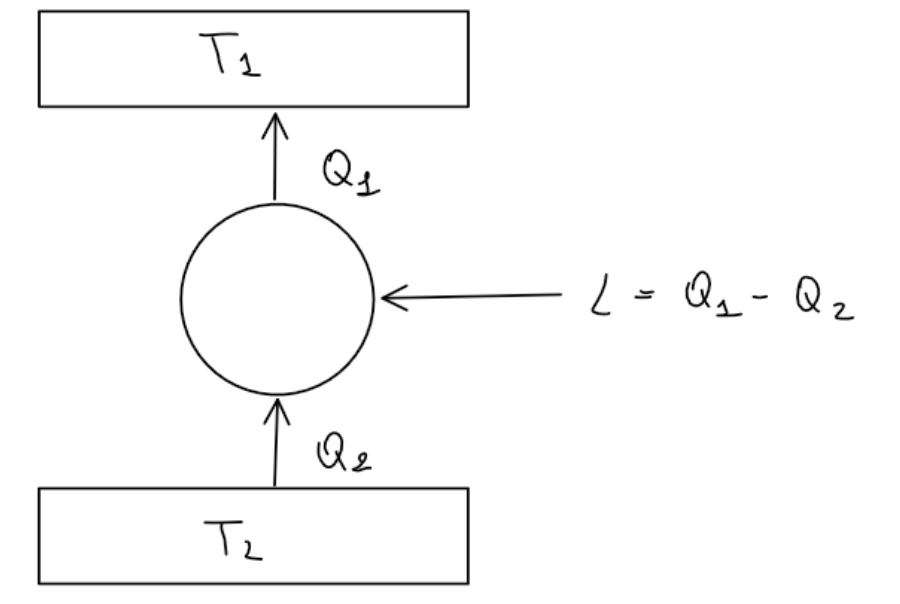
\includegraphics[width=0.3\columnwidth]{cicloinverso.png}
		\caption{Ciclo inverso}
	\end{center}
\end{figure}

\subsubsection{Ciclo frigorifero}\index{Ciclo inverso! frigorifero}
Il rendimento del ciclo frigorifero $\eta_F={Q_2\over L}=\frac{T_{2}}{T_{1}-T_{2}}-\frac{\tau}{L} \cdot \frac{T_{1} T_{2}}{T_{1}-T_{2}}$.

Il secondo termine contiene le irreversibilità.
Il diagramma nel piano Ts è un rettangolo.

\subsubsection{Pompa di calore}\index{Ciclo inverso! pompa di calore}

Il rendimento della pompa di calore $\eta_{PC}={Q_1\over L}=\frac{T_{1}}{T_{1}-T_{2}}-\frac{\tau}{L} \cdot \frac{T_{1} T_{2}}{T_{1}-T_{2}}$

Il secondo termine contiene le irreversibilità, se la trasformazione è reversibile $\tau=0$.
Il diagramma Ts è lo stesso rettangolo del ciclo frigorifero. 

\subsection{Diagrammi termodinamici}

\subsubsection{Isobare nel $Ts$}

Partendo dal differenziale esatto dell'entalpia e dalla \eqref{eq:entalpiaentropia} e considerando che per un'isobara $dp=0$, abbiamo che: $d h=\left(\frac{\partial h}{\partial T}\right)_{p} d T=c_{p} d T=T d s$.
Calore specifico isobaro:
\begin{equation}
	\left(\frac{\partial h}{\partial T}\right)_{p}=c_{p}
	\label{eq:calore_specifico_isobaro}
\end{equation}
\myequations{Calore specifico isobaro}

Possiamo misurare le derivate parziali (sono quantità fisiche): $\left(\frac{\partial T}{\partial s}\right)_{p}=\frac{T}{c_{p}}>0$

Oss: se $cp\approx cost \Longrightarrow$ la pendenza cresce con la temperatura $T$.  Allora la curva isobara ha la concavità verso l’alto,$\rightarrow$ curva crescente

\begin{figure}[H]
	\begin{center}
		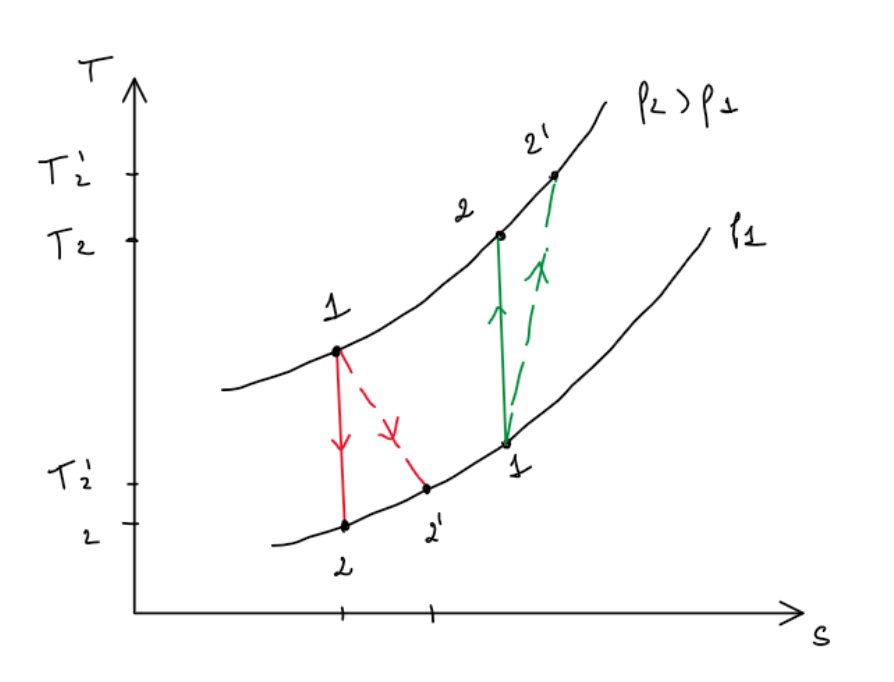
\includegraphics[width=0.4\columnwidth]{isobara_Ts.png}
		\caption{Isobara}
	\end{center}
\end{figure}

\begin{itemize}
	\item Espansore, in \textcolor{red}{rosso}, tratteggiata la trasformazione reale irreversibile in cui è presente $\Delta s_s$. 
	\item Compressore, in \textcolor{green}{verde}, discorso analogo
\end{itemize}
In entrambi i casi la temperatura del caso irreversibile è più alta del caso reversibile. Nel caso irreversibile si ottiene meno lavoro che viene dissipato sotto forma di calore per le irreversibilità. 
\newline
Nel diagramma $Ts$ l'isobara a pressione maggiore si trova sopra.

Considerando \eqref{eq:sistemi_aperti_coefficienti} se la trasformazione è isoentropica e  sfruttando \eqref{eq:coeff_dilatazione_isobara} abbiamo:
\begin{equation}
\frac{c_{p}}{T} d T=\left(\frac{\partial v}{\partial T}\right)_{p} d p \Rightarrow \frac{d T}{d p}=\frac{v \beta T}{c_{p}}>0
\end{equation}
 Quindi, muovendosi lungo un’isoentropica, ad un aumento di temperatura corrisponde un aumento di pressione.
 \newline
 
 Abbiamo anche la pendenza dell'isocora è maggiore di quella dell'isobara.
Vedi pg. \pageref{relazioni_cv_cp}.





\subsubsection{Isobare nel diagramma $hs$}

Prendiamo il differenziale dell'entalpia e ricordiamo  \eqref{eq:entalpiaentropia} e per un'isobara $dp=0$, abbiamo che: $d h=\left(\frac{\partial h}{\partial s}\right)_{p} d s=T d s \Rightarrow\left(\frac{\partial h}{\partial s}\right)_{p}=T$ 
La pendenza dell'isobara nel piano $hs$ è $T$.
Oss: se $cp\approx cost \Longrightarrow$ la pendenza cresce con la temperatura $T$.  Allora la curva isobara ha la concavità verso l’alto,$\rightarrow$ curva crescente


\begin{figure}[H]
	\begin{center}
		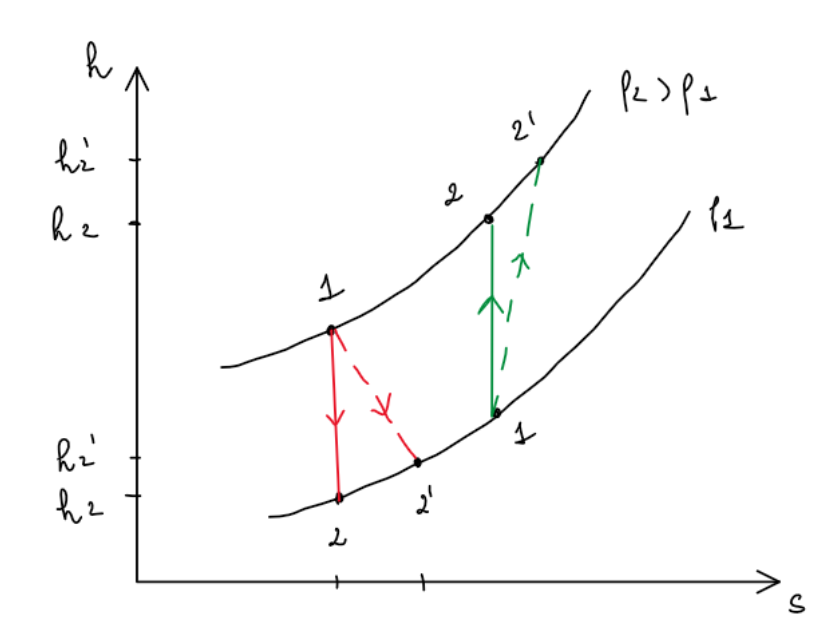
\includegraphics[width=0.4\columnwidth]{isobara_hs.png}
		\caption{Isobara}
	\end{center}
\end{figure}

\begin{itemize}
	\item Espansore, in \textcolor{red}{rosso}, tratteggiata la trasformazione reale irreversibile in cui è presente $\Delta s_s$. 
	\item Compressore, in \textcolor{green}{verde}, discorso analogo
	\item Valvola di laminazione, l'entalpia di ingresso è uguale a quella di uscita (orizzontale). È irreversibile e arriva ad una pressione di uscita inferiore. 
\end{itemize}
In entrambi i casi l'entalpia del caso irreversibile è più alta del caso reversibile. 

\subsection{Proprietà della sostanze}

\subsubsection{Gas perfetti e coefficienti}
Obbediscono all'equazione di stato dei gas perfetti 
\begin{equation}
	pv=RT
		\label{eq:gas_perfetti}
\end{equation}
\myequations{Legge di stato dei gas perfetti}

La costante specifica di gas $R={R_u\over p.m.}$

Note le funzioni termodinamiche generiche, possiamo procedere come se fossero espressioni matematiche, tutto quello che otteniamo ha un significato fisico ed è rappresentato da grandezze misurabili.

Sostanza che scambia calore e subisce una variazione di temperatura ha una corrispondente variazione del suo volume specifico: $d v=\left(\frac{\partial v}{\partial T}\right)_{p} d T+\left(\frac{\partial v}{\partial p}\right)_{T} d p$. Da cui la quantità misurabile, il \textbf{coefficiente di dilatazione isobara}:
\begin{equation}
	\left(\frac{\partial v}{\partial T}\right)_{p} \frac{1}{v}=\beta
\label{eq:coeff_dilatazione_isobara}
\end{equation}

E il \textbf{coefficiente di compressione isoterma}:
\begin{equation}
	\left(\frac{\partial v}{\partial p}\right)_{T}\left(-\frac{1}{v}\right)=\gamma
\end{equation}

Se le variazioni di volume specifico avvengono a sezione costante, possiamo dividere per la sezione e ottenere il \textbf{coefficiente di dilatazione lineare}:
\begin{equation}
\frac{1}{x}\left(\frac{\partial x}{\partial T}\right)_{p}=\alpha
\end{equation}

Quindi l'equazione differenziale del volume specifico: 
\begin{equation}
	d v=\beta v d T-\gamma v d p
	\label{eq:differenziale_volume_specifico}
\end{equation}
\myequations{Equazione differenziale del volume specifico}


Abbiamo visto le relazioni tra $c_v$ e $c_p$, cioè \eqref{eq:cp-cv} e \eqref{eq:cp/cv}, e  \eqref{eq:cp-cv-R}  \eqref{eq:cp/cv-k} e che questi, per i gas perfetti, dipendono solo da $T$. Inoltre vale che 
\begin{equation}
	\begin{aligned}
d u=c_{v}(T) d T\\
dh=c_{p}(T) d T
	\end{aligned}
\end{equation}

E possiamo trovare il \textbf{coefficiente di dilatazione isobara $\beta$} per i gas perfetti \begin{equation}
\beta=\frac{1}{v}\left(\frac{\partial v}{\partial T}\right)_{p}=\frac{1}{v} \cdot \frac{R}{P}=\frac{R}{R T}=\frac{1}{T} \Rightarrow \beta=\frac{1}{T}
\end{equation}
\newline
\subsubsection{Conferma sperimentale $d u=c_{v}(T) d T$ e $dh=c_{p}(T) d T$}

Nell'esperienza di Joule c'è un gas che compie una trasformazione in cui varia il suo volume e la temperatura rimane costante.

\begin{figure}[H]
	\begin{center}
		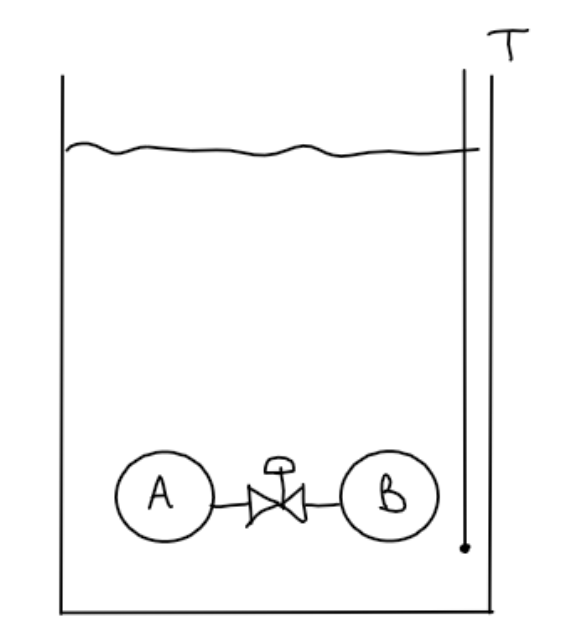
\includegraphics[width=0.3\columnwidth]{confermasperimentale.png}
	\end{center}
\end{figure}

Quindi applichiamo il primo principio della termodinamica per sistemi chiusi:
\begin{itemize}
\item non scambia lavoro
\item $q=0$ temperatura costante
\item velocità nulla
\item non cambia la quota del baricentro
\end{itemize}

$\Longrightarrow$ $du=0$ e il suo differenziale esatto $ u(v, T) \rightarrow d u=\left(\frac{\partial u}{\partial v}\right)_{T} d v+\left(\frac{\partial u}{\partial T}\right)_{v} d T$ in cui c'è una variazione di volume ($dv\neq 0$) otteniamo che $\left(\frac{\partial u}{\partial v}\right)_{T}=0$. Ovvero abbiamo confermato che \underline{$u$ è funzione solo della temperatura} e non del volume specifico.
\newline

Considerando l'esperienza di Joule-Thompson 

\begin{figure}[H]
	\begin{center}
		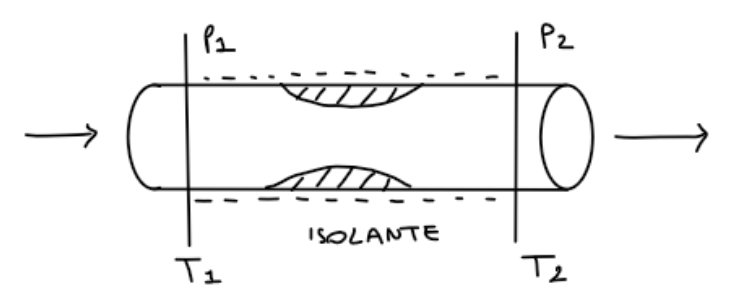
\includegraphics[width=0.3\columnwidth]{jouleT.png}
	\end{center}
\end{figure}

Applichiamo il primo principio della termodinamica per sistemi aperti e con considerazioni analoghe alle precedenti $\Longrightarrow$ $dh=0$.  Ne facciamo il differenziale: $h(p, T) \rightarrow d h=\left(\frac{\partial h}{\partial T}\right)_{p} d T+\left(\frac{\partial h}{\partial p}\right)_{T} d p$ e, considerando che c'è un $dp\neq 0$, troviamo che $\left(\frac{\partial h}{\partial p}\right)_{T}=0$. Ovvero abbiamo confermato che \underline{$h$ è funzione solo della temperatura} e non della pressione.
\newline

In condizioni reali però $dT\neq 0$ e se un gas espande si ottiene una variazione della temperatura (diminuzione) e quindi $h=h\left(p,T\right)$. 

Possiamo rappresentare l'esperienza in un diagramma $pT$ rappresentando esperienze successive con pressioni sempre più basse otteniamo un andamento inizialmente crescente e poi decrescente. Unendo i massimi troviamo la curva dove $c_{JT}=0$. 

In particolare, il \textbf{coefficiente di Joule-Thompson}:
\begin{equation}
C_{J T}=\left.\left(\frac{\Delta T}{\Delta p}\right)\right|_{h}=-\frac{\left(\frac{\partial h}{\partial p}\right)_{T}}{c_{p}}
\end{equation}


\begin{figure}[H]
	\begin{center}
		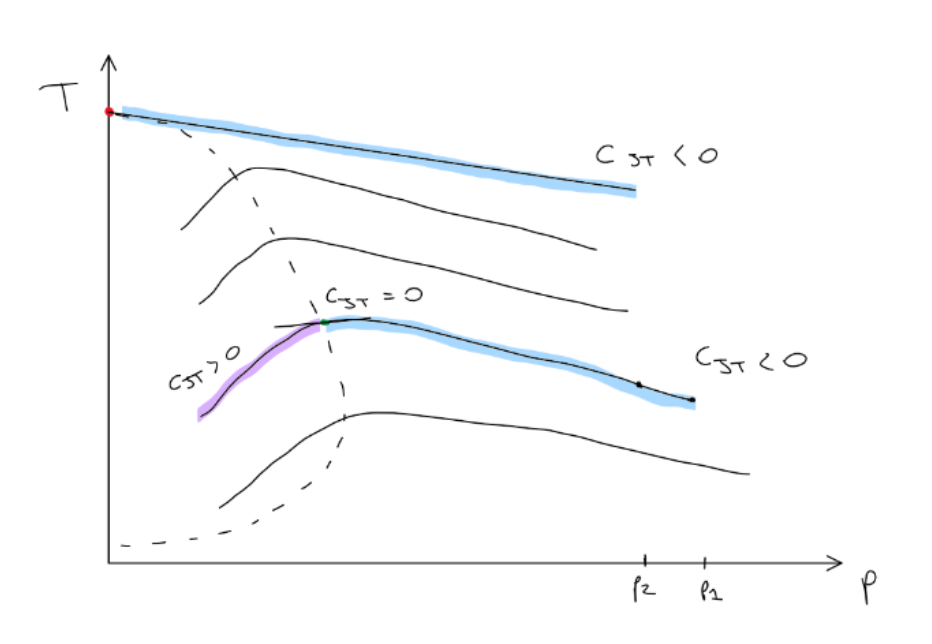
\includegraphics[width=0.4\columnwidth]{jt-pt.png}
		\caption{Esperienza Joule-Thompson sul $pT$}
	\end{center}
\end{figure}

Conviene leggerle dal dx verso sx (nell'esperienza andiamo da $p$ maggiori a $p$ minori). 

Di solito, un gas che si espande si raffredda, ma questo vale nel tratto a sx del massimo. Esiste una temperatura in cui$ c_{JT}=0$ , nota come \textbf{temperatura limite} o di inversione. A partire da questa il gas che si espande si riscalda sempre.

Sperimentalmente si misura un $\Delta T/\Delta p$ e si ottiene un proporzionalità a $\Delta p/T^2$ come:  $ c_{J T}=\frac{\Delta T}{\Delta p}=\frac{\Delta p}{T^{2}} \cdot k \rightarrow\left\{\begin{array}{l}
	\text { se } k>0, \Delta T>0 \\
	\text { se } k<0, \Delta T<0
\end{array}\right.$ (legge empirica).


\subsubsection{Calore specifico}

\begin{equation}
c={dq\over dT}
\end{equation}

Dipende dalla trasformazione in quanto $dq$ non è differenziale esatto.
\begin{itemize}
\item Se è adiabatica $dq=0\Rightarrow c=0$
\item Se è isoterma $dT=0$ ma $dq=0\Rightarrow c=\pm \infty$
\end{itemize}

\textbf{Sistemi chiusi}
Partendo dal primo principio della termodinamica e considerando una trasformazione reversibile (per cui $dl=pdv$), otteniamo: $dq=du+pdv$.
Sostituendo nel calore specifico otteniamo $c=\frac{d q}{d T}=\frac{d u}{d T}+p \frac{d v}{d T}$.
Quindi il differenziale esatto di $u=u(T,v)$ e possiamo dividere per $dT$ e sostituire nell'espressione del calore specifico, poi moltiplichiamo il tutto per $dT$:
\begin{equation}
dq=\left(\frac{\partial u}{\partial T}\right)_{v} d T+\left[p+\left(\frac{\partial u}{\partial v}\right)_{T}\right]{dv}
\end{equation}

Se la trasformazione è isocora allora otteniamo il \textbf{calore specifico a volume costante} 
\begin{equation}
c_{v}=\left(\frac{\partial u}{\partial T}\right)_{v}
\label{eq:cv}
\end{equation}
\myequations{Calore specifico a volume costante}
In queste condizioni vale che $dq=c_vdT$ e quindi possiamo misurarlo come $c_{v}=\left.\frac{d q}{d T}\right|_{v}=\left.\frac{q}{\Delta T}\right|_{v}$

Se la trasformazione è isoterma allora otteniamo il \textbf{calore specifico di dilatazione isoterma} 
\begin{equation}
c_{d}=\left[p+\left(\frac{\partial u}{\partial v}\right)_{T}\right] 
\end{equation}
\myequations{Calore specifico di dilatazione isoterma }
In queste condizioni vale che $dq=c_ddv$ e allora possiamo misurarlo: $c_{d}=\left.\frac{d q}{d v}\right|_{T}$. Possibile solo nei passaggi di stato.

Quindi per i \textbf{sistemi chiusi} vale che:
\begin{equation}
dq=c_vdT+c_ddv 
\label{eq:calore_sistemi_chiusi}
\end{equation}
\myequations{Calore per sistemi chiusi}
E  il calore specifico possiamo esprimerlo come:
\begin{equation}
c=c_v+c_d{dv\over dT}
\end{equation}
\myequations{Calore specifico per sistemi chiusi}


\textbf{Sistemi aperti}
Partiamo dal primo primo principio della termodinamica per sistemi aperti e supponendo la trasformazione reversibile ($dl_f=-vdp$). Otteniamo che $dq=dh-vdp$. Allora sostituendo nella relazione del calore specifico otteniamo $c=\frac{d q}{d T}=\frac{d h}{d T}-v \frac{d p}{d T}$. Quindi possiamo fare il differenziale esatto di $h=h(p,T)$ e dividere per $dT$. Poi sostituiamo nell'espressione del calore specifico e moltiplichiamo per $dT$, quindi otteniamo:
\begin{equation}
d q=\left(\frac{\partial h}{\partial T}\right)_{p} d T+\left[\left(\frac{\partial h}{\partial p}\right)_{T}-v\right] d p
\end{equation}


Se la trasformazione è isobara allora otteniamo il \textbf{calore specifico a pressione costante} 
\begin{equation}
	c_{p}=\left(\frac{\partial h}{\partial T}\right)_{p}
	\label{eq:cp}
\end{equation}
\myequations{Calore specifico a pressione costante}
In queste condizioni vale che $dq=c_pdT$ e quindi possiamo misurarlo come $c_{p}=\left.\frac{d q}{d T}\right|_{p}=\left.\frac{q}{\Delta T}\right|_{p}$

Se la trasformazione è isoterma allora otteniamo il \textbf{calore specifico di comprimibilità isoterma} 
\begin{equation}
	c_{c}=\left[\left(\frac{\partial h}{\partial p}\right)_{T}-v\right]
\end{equation}
\myequations{Calore specifico di comprimibilità isoterma }
In queste condizioni vale che $dq=c_cdp$ e allora possiamo misurarlo: $c_{c}=\left.\frac{d q}{d p}\right|_{T}$. Possibile solo nei passaggi di stato.

Quindi per i \textbf{sistemi aperti} vale che:
\begin{equation}
	dq=c_pdT+c_cdp 
	\label{eq:calore_sistemi_aperti}
\end{equation}
\myequations{Calore per sistemi aperti}
E  il calore specifico possiamo esprimerlo come:
\begin{equation}
	c=c_p+c_c{dp\over dT}
\end{equation}
\myequations{Calore specifico per sistemi aperti}

\subsubsection{Equazioni di Maxwell}

Introduciamo due nuove grandezze funzioni di stato:
\begin{itemize}
\item Energia libera di Gibbs $e_u=u-Ts$
\item Entalpia libera di Helmotz $e_h=h-Ts$
\end{itemize}

Possiamo farne i differenziali esatti (considerando anche \eqref{eq:energiainternaentropia} e \eqref{eq:entalpiaentropia}) otteniamo:
\begin{itemize}
	\item $de_u=-pdv-sdT$
	\item $de_h=vdp-sdT$
\end{itemize}

Nei passaggi di tasto (isotermobariche) abbiamo $de_h=0$.

Per un'isoterma abbiamo $p d v=-d e_{u} \rightarrow \int_{1}^{2} p d v=l_{21}=e_{u 1}-e_{u 2}$ quindi riconduciamo il calcolo del lavoro ad una variazione di una funzioni di stato. 

Applicando il teorema di Swartz all'energia libera, entalpia libera, energia interna e entalpia otteniamo le quattro \textbf{equazioni di Maxwell}
\begin{equation}
\left.\begin{aligned}
	-\left(\frac{\partial p}{\partial T}\right)_{v}&=-\left(\frac{\partial s}{\partial v}\right)_{T} \\
	\left(\frac{\partial v}{\partial T}\right)_{p}&=-\left(\frac{\partial s}{\partial p}\right)_{T} \\
	\left(\frac{\partial T}{\partial v}\right)_{s}&=-\left(\frac{\partial p}{\partial s}\right)_{v} \\
	\left(\frac{\partial T}{\partial p}\right)_{s}&=\left(\frac{\partial v}{\partial s}\right)_{p}
\end{aligned}\right.
\end{equation}
\myequations{Equazioni di Maxwell}

Cerchiamo delle espressioni analitiche per $c_d$ e $c_c$.
Dalla definizione di entropia $ds=dq/T$ sostituiamo la definizione di calore \eqref{eq:calore_sistemi_chiusi}. Poi possiamo farne il differenziale esatto $ds=ds(T,v)$ e otteniamo:
\begin{equation}
d s=\left(\frac{\partial s}{\partial T}\right)_{v} d T+\left(\frac{\partial s}{\partial v}\right)_{T} d v
\end{equation}

\begin{itemize}
\item Trasformazioni isocore $c_{v}=\left(\frac{\partial s}{\partial T}\right)_{v} T$
\item Trasformazioni isoterme $c_{d}=\left(\frac{\partial s}{\partial v}\right)_{T} T$
\end{itemize}

Quindi dalla prima equazione di Maxwell: 
\begin{equation}
c_{d}=T\left(\frac{\partial p}{\partial T}\right)_{v}
\end{equation}

Nota l'equazione di stato possiamo calcolarlo analiticamente. 
\newline


Dalla definizione di entropia $ds=dq/T$ sostituiamo la definizione di calore \eqref{eq:calore_sistemi_aperti}. Poi possiamo farne il differenziale esatto $ds=ds(T,p)$ e otteniamo:
\begin{equation}
d s=\left(\frac{\partial s}{\partial T}\right)_{p} d T+\left(\frac{\partial s}{\partial p}\right)_{T} d p
\end{equation}

\begin{itemize}
	\item Trasformazioni isobare $c_{p}=T\left(\frac{\partial s}{\partial T}\right)_{p}$
	\item Trasformazioni isoterme $c_{c}=T\left(\frac{\partial s}{\partial p}\right)_{T}$
\end{itemize}

Quindi dalla seconda equazione di Maxwell: 
\begin{equation}
c_{c}=-T\left(\frac{\partial v}{\partial T}\right)_{p}
\end{equation}
Nota l'equazione di stato possiamo calcolarlo analiticamente. 
\newline

In conclusione: 

\begin{multicols}{2}
	\begin{center}
\textbf{Sistemi chiusi}
	\end{center}

\begin{equation}
\begin{aligned}
	&d q=c_{v} d T+T\left(\frac{\partial p}{\partial T}\right)_{v} d v \\
	&d u=c_{v} d T+\left[T\left(\frac{\partial p}{\partial T}\right)_{v}-p\right] d v \\
	&d s=\frac{c_{v}}{T} d T+\left(\frac{\partial p}{\partial T}\right)_{v} d v
\end{aligned}
	\label{eq:sistemi_chiusi_coefficienti}
\end{equation}


\begin{center}
\textbf{Sistemi aperti}
\end{center}
\begin{equation}
\begin{aligned}
	&d q=c_{p} d T-T\left(\frac{\partial v}{\partial T}\right)_{p} d p \\
	&d h=c_{p} d T+\left[v-T\left(\frac{\partial v}{\partial T}\right)_{p}\right] d p \\
	&d s=\frac{c_{p}}{T} d T-\left(\frac{\partial v}{\partial T}\right)_{p} d p 
\end{aligned}
\label{eq:sistemi_aperti_coefficienti}
\end{equation}




\end{multicols}

\subsubsection{Relazioni tra calori specifici}\label{relazioni_cv_cp}

 Consideriamo l'ultima da \eqref{eq:sistemi_chiusi_coefficienti} se la trasformazione è isocora abbiamo la pendenza dell'isocora sul piano $Ts$:
 \begin{equation}
d s=\left.\frac{c_{v}}{T} d T \Rightarrow \frac{d T}{d s}\right|_{v}=\left.\frac{T}{c_{v}}\right|_{v}
 \end{equation}

Considerando  l'ultima da \eqref{eq:sistemi_aperti_coefficienti} se la trasformazione è isobara otteniamo la pendenza dell'isobara sul piano $Ts$:
\begin{equation}
d s=\left.\frac{c_{p}}{T} d T \Rightarrow \frac{d T}{d s}\right|_{p}=\left.\frac{T}{c_{p}}\right|_{p}
\end{equation}

Poiché $c_p>c_v$ (lo dimostreremo) la pendenza dell'isobara è minore dell'isocora.
\newline

Considerando  l'ultima da \eqref{eq:sistemi_aperti_coefficienti} esplicitiamo $c_p$ e dall'ultima da \eqref{eq:sistemi_chiusi_coefficienti} esplicitiamo $c_v$. Dalla loro differenza otteniamo: 
\begin{equation}
	c_{p}-c_{v}=\left(\frac{\partial v}{\partial T}\right)_{p} T \frac{d p}{d T}+\left(\frac{\partial p}{\partial T}\right)_{v} T \frac{d v}{d T}
\end{equation}

Consideriamo il differenziale esatto di $p=p(T,v)$ e dividiamo per $dT$ allora sostituiamo in $c_p-c_v$ e otteniamo:

\begin{equation}
	c_{p}-c_{v}=\left(\frac{\partial v}{\partial T}\right)_{p} T\left(\frac{\partial p}{\partial T}\right)_{v}
		\label{eq:cp-cv}
\end{equation}
Avendo semplificato grazie al teorema dei differenziali esatti.
\newline

Oss: per i gas perfetti otteniamo $p v=R T \rightarrow\left(\frac{\partial p}{\partial T}\right)_{v}=\frac{R}{v}$ e $\left(\frac{\partial v}{\partial p}\right)_{T}=-\frac{R T}{p^{2}}$.
Quindi otteniamo \begin{equation}
	c_{p}-c_{v}=T \frac{R^{2}}{v^{2}} \cdot \frac{R T}{p^{2}}=R \Rightarrow {c}_{{p}}-{c}_{v}=\boldsymbol{R}
		\label{eq:cp-cv-R}
\end{equation}
\newline
Se è isoentropica dalle ultime di  \eqref{eq:sistemi_aperti_coefficienti} e  \eqref{eq:sistemi_chiusi_coefficienti} possiamo esplicitare $c_p$ e $c_v$ e considerarne il rapporto: \begin{equation}
\frac{c_{p}}{c_{v}}=-\frac{\left(\frac{\partial v}{\partial T}\right)_{p}}{\left(\frac{\partial p}{\partial T}\right)_{v}} \cdot \frac{\left(\frac{\partial p}{\partial T}\right)_{s}}{\left(\frac{\partial v}{\partial T}\right)_{s}}=\left(\frac{\partial v}{\partial p}\right)_{T}\left(\frac{\partial p}{\partial v}\right)_{s}
	\label{eq:cp/cv}
\end{equation}
Dove ho semplificato il $\partial T$

Inoltre $\frac{\left(\frac{\partial v}{\partial T}\right)_{p}}{\left(\frac{\partial p}{\partial T}\right)_{v}}=-\left(\frac{\partial v}{\partial p}\right)_{T}$ per Swartz (il prodotto dei 3 è $-1$) . 
\newline
Oss: nei gas perfetti: 
$p v=R T \rightarrow\left(\frac{\partial v}{\partial p}\right)_{T}=-\frac{R T}{p^{2}}$
e quindi per le trasformazioni \textbf{isoentropiche} \begin{equation}
	pv^k=\operatorname{cost}
\end{equation}

Facendone la derivata possiamo ricavare 
\begin{equation}
\left(\frac{\partial p}{\partial v}\right)_{s}=-k p \frac{v^{k-1}}{v^{k}}=-k \frac{p}{v}
\end{equation}

E allora:

\begin{equation}
\frac{c_{p}}{c_{v}}=+\frac{R T}{p^{2}} \cdot k \frac{p}{v}=\frac{R T}{p v} k=k \Rightarrow \frac{\boldsymbol{c}_{\boldsymbol{p}}}{\boldsymbol{c}_{v}}=\boldsymbol{k}
	\label{eq:cp/cv-k}
\end{equation}

\subsubsection{Dipendenza di $c_v$ da $v$}

Considerando la definizione di $c_v$ \eqref{eq:cv} deriviamolo rispetto $v$ a $T$ costante e invertiamo l'ordine di integrazione. Quindi ricordando l'espressione di $du$ per i sistemi chiusi \eqref{eq:sistemi_chiusi_coefficienti} calcoliamo il $\left(\partial u\over \partial v\right)_T$, sostituiamo e otteniamo: 
\begin{equation}
\left(\frac{\partial c_{v}}{\partial v}\right)_{T}=T\left(\frac{\partial^{2} p}{\partial T^{2}}\right)_{v}
\end{equation}
\myequations{Relazione tra $c_v$ e $v$}

\subsubsection{Dipendenza di $c_p$ da $p$}

Considerando la definizione di $c_p$ \eqref{eq:cp} deriviamolo rispetto $p$ a $T$ costante e invertiamo l'ordine di integrazione. Quindi ricordando l'espressione di $dh$ per i sistemi chiusi \eqref{eq:sistemi_aperti_coefficienti} calcoliamo il $\left(\partial h\over \partial p\right)_T$, sostituiamo e otteniamo: 
\begin{equation}
	\left(\frac{\partial c_{p}}{\partial p}\right)_{T}=-T\left(\frac{\partial^{2} v}{\partial T^{2}}\right)_{p}
\end{equation}
\myequations{Relazione tra $c_p$ e $p$}

\subsection{Teorema di Guoj-Stodola}

\begin{figure}[H]
	\begin{center}
		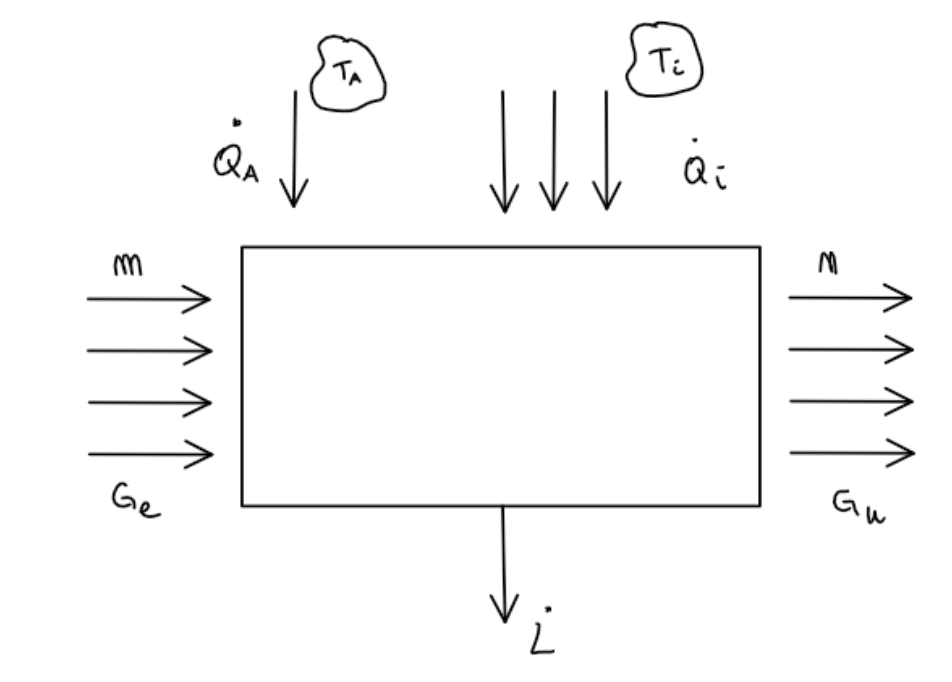
\includegraphics[width=0.3\columnwidth]{guoj.png}
	\end{center}
\end{figure}

Applicando il primo principio e considerando che $\dot{Q}=\dot{Q}_{A}+\sum_{i=1}^{m} \dot{Q}_{i}$ possiamo applicare il secondo principio tenendo conto delle irreversibilità $\frac{\dot{Q}}{T}=\Delta S-\Delta \mathrm{s}_{\mathrm{S}}$, otteniamo:
\begin{equation}
\dot{L}=\underbrace{\sum_{i} \dot{Q}_{l}\left(1-\frac{T_{A}}{T_{i}}\right)+\sum G_{e}\left(h_{e}-T_{A} s_{e}+e_{c e}+e_{p e}\right)-\sum G_{u}\left(h_{u}-T_{A} s_{u}+e_{c u}+e_{p u}\right)}_{\dot{L}_{\max}}-T_{A} \Delta s_{s}
\end{equation}
\myequations{Teorema di Guoi-Stodola}

Si osservi che il lavoro ottenibile per un sistema aperto è massimo quando non ci sono irreversibilità. Questo lavoro dipende dai calori scambiati con le sorgenti, dall'entalpia e dal termine $T_As$.
\newline

Nel caso di \textbf{sistemi chiusi} si torna alla macchina motrice di Watt (e Carnot se reversibili) e spariscono i termini legati alle correnti entranti/uscenti. 
$ \dot{L}=\sum_{i} \dot{Q}_{l}\left(1-\frac{T_{A}}{T_{i}}\right)$.	
	In particolare, con una sola sorgente, abbiamo l'\textbf{exergia} del sistema chiuso
	\begin{equation}
	L_{\max }^{\cdot}=\dot{Q}_{l}\left(1-\frac{T_{A}}{T_{i}}\right)=\dot{E}_{x}
\end{equation}
\myequations{Exergia del sistema chiuso}

	È il lavoro massimo ottenuto dal sistema chiuso che scambia calore con una sola sorgente	
Facciamo il diagramma dell’exergia per unità di calore scambiato in modulo, in funzione della temperatura $T_1$ della sorgente, fissata la temperatura ambiente $T_a$ in cui identifichiamo il ciclo diretto ( $\frac{\left|E_{x}\right|}{\left|\dot{Q_{1}}\right|}$ aumenta verso la saturazione) e ciclo inverso ($\frac{\left|E_{x}\right|}{\left|\dot{Q_{1}}\right|}$ aumenta in maniera inversa).

\begin{figure}[H]
	\begin{center}
		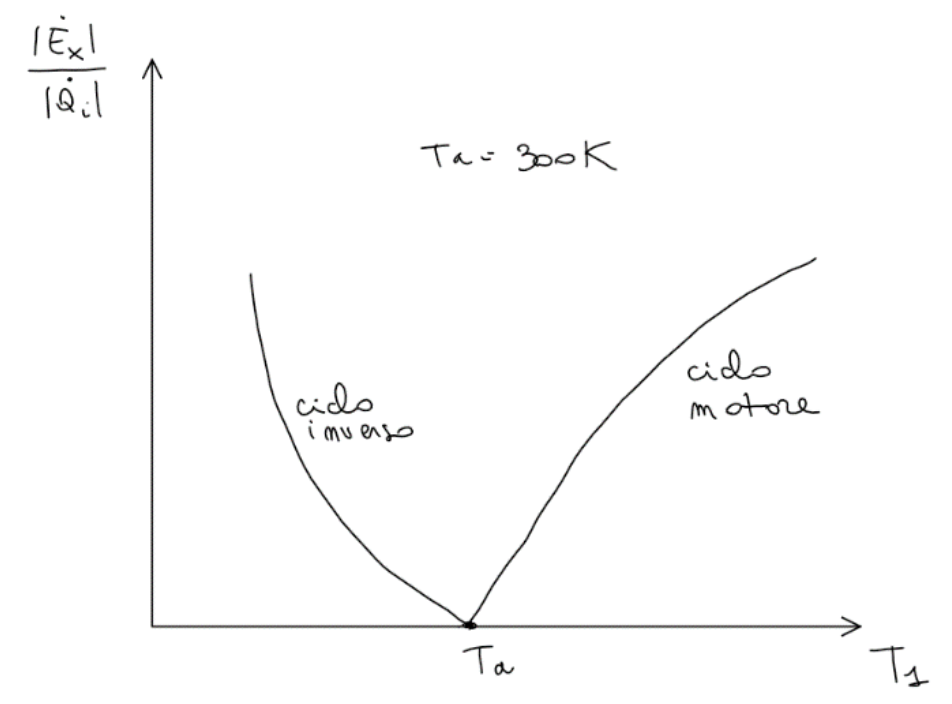
\includegraphics[width=0.5\columnwidth]{diagrammaexergia.png}
	\end{center}
\caption{Diagramma dell'exergia per unità di calore}
\end{figure}

\newpage
\section{Tesine}

\newpage
\section{Indici}





\listoffigures
\addcontentsline{toc}{subsection}{\listfigurename}

\newpage
\listoftables
\addcontentsline{toc}{subsection}{\listtablename}
\newpage
\listofmyequations
\addcontentsline{toc}{subsection}{\listequationsname}
\newpage
\addcontentsline{toc}{subsection}{Indice analitico}
\printindex
\newpage








\end{document}